\documentclass[a4paper,12pt]{article} 
\usepackage[T2A]{fontenc}			
\usepackage[utf8]{inputenc}			
\usepackage[english,russian]{babel}	
\usepackage{amsmath,amsfonts,amssymb,amsthm,mathtools} 
\usepackage[colorlinks, linkcolor = blue]{hyperref}
\usepackage{upgreek}
\usepackage[left=2cm,right=2cm,top=2cm,bottom=3cm,bindingoffset=0cm]{geometry}
\usepackage{multirow}
\usepackage{graphicx}
\usepackage{xcolor}
\usepackage{multirow}
\usepackage{pgfplots}
\usepackage{pgfplotstable}
\pgfplotsset{compat=1.9}

\pgfplotstableset{ %
        create on use/SquareLight/.style={
                create col/expr={\thisrow{Dark}}}
}

\author{Шелихов Дмитрий\\Группа Б01-305}

\title{\textbf{Работа 3.7.1\\Скин-эффект в полом цилиндре}} 
\date{\today}

\begin{document} 

\maketitle

\textbf{Цель работы:} исследовать явление проникновения переменного магнитного поля в медный полый цилиндр. \\
\par\textbf{В работе используются:} генератор сигналов АКИП-3420, соленоид, намотанный на полый цилиндрический каркас, медный экран в виде полого цилиндра, измерительная катушка, амперметр, вольтметр, двухканальный осциллограф GOS-620, RLC-метр. \\

\par\textbf{Теоретические сведения}\\

Считаем цилиндр достаточно длинным, так что в нем можно пренебречь краевыми эффектами. Тогда магнитное поле $\vec{H}$ всюду направлено по оси системы Oz, а вихревое электрическое поле $\vec{E}$ будет всюду перпендикулярно радиусу. (линии поля образуют соосные окружности)

\begin{figure}
\center{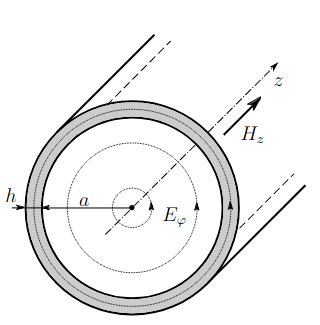
\includegraphics[width=.6\textwidth]{1.png}}[H]
\caption{Электрическое и магнитное поле в тонкостенном цилиндре}
\end{figure}

Все величины считаем колеблющимися по гармоническому закону с некоторой частотой $\omega$, задаваемой частотой колебания тока в соленоиде. Тогда: 

$$H_z = H(r)e^{i\omega t}, E_z = E(r)e^{i\omega t}$$

На границе цилиндра должны быть непрерывны касательные к поверхности компоненты как $\vec{E}$, так и $\vec{H}$ => E(r) и H(r) непрерывны во всей исследуемой области. \\
Пусть длинный полый цилиндр имеет радиус a и толщину стенки h << a. Последнее условие позволяет для описания поля внутри стенки ограничиться одномерным приближением. При этом для полного решения задачи необходимо вычислить и распределение поля внутри цилиндра. \\
Внутри цилиндра ток отсутсвует => магнитное поле там является однородным $H_z(r,t) = H_1e^{i\omega t}$, где $H_1$ = const - амплитуда поля на внутренней поверхности цилиндра. Для нахождения вихревого электрического поля воспользуемся законом электромагнитной индукции в интегральной форме: 
$$E_{\varphi} \cdot 2\pi r = - {\mu}_0\pi r^2 \cdot \frac{dH_z}{dt} \rightarrow E(r) = -\frac{1}{2}{\mu}_0 r \cdot i\omega H_1$$. 

Откуда получаем связь амплитуд колебаний электрического и магнитного полей на внутренней (r = a) границе цилиндра: 

$$ E_1 = -\frac{1}{2}i\omega a{\mu}_0 H_1 $$

\begin{figure}[htp]
\center{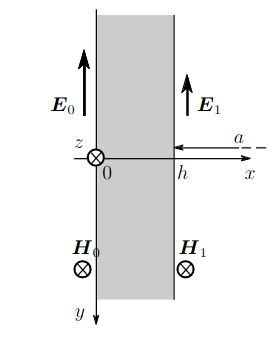
\includegraphics[width=.4\textwidth]{2.png}}
\caption{Поле в стенке цилиндра}
\end{figure}

Поле внутри тонкой стенки цилиндра описывается уравнением скин-эффекта в плоском случае:
$$\frac{d^2 H}{dx^2} = i\omega \sigma {\mu}_0 H$$

Где для медного цилиндра $\mu \approx$ 1. 

Граничные условия: 

$$H(0) = H_1, H(h) = H_1$$. 

Решением дифференциального уравнения скин-эффекта с учетом граничных условий при x = h является: 

$$H_1 = \frac{H_0}{ch(\alpha h) + \frac{1}{2}\alpha a sh(\alpha h)}$$

где $\alpha = \frac{\sqrt{2}}{\delta}e^{i\pi/4}$, $\delta = \sqrt{\frac{2}{\omega \sigma {\mu}_0}}$ - глубина скин-слоя. 

Предельные случаи: \\ 

1) При малых частотах $\delta >> h$, тогда $|\alpha h|$ << 1, поэтому $ch\alpha h \approx 1$, $sh \alpha h \approx \alpha h$ и 

$$H_1 \approx \frac{H_0}{1+i\frac{ah}{{\delta}^2}}$$

Отношение модулей амплитуд: 

$$\frac{|H_1|}{|H_0|} = \frac{1}{\sqrt{1 + \frac{1}{4}(ah\sigma{\mu}_0\omega})^2}$$

При этом колебания $H_1$ отстают по фазе от $H_0$ на угол $\psi$:

$$tg(\psi) = \frac{ah}{{\delta}^2}$$

2) При достаточно больших частотах $\delta$ << h. Тогда sh($\alpha h$) $\approx$ ch($\alpha h$) $\approx$ $\frac{1}{2}e^{\alpha h}$.

Отношение амплитуд: 

$$\frac{H_1}{H_0} = \frac{4e^{-\alpha h}}{\alpha a} = \frac{2\sqrt \delta}{a} \cdot e^{-\frac{h}{\delta}}e^{-i(\frac{\pi}{4} + \frac{h}{\delta})}$$. 

Запаздывание поля внутри, чем поля снаружи на: 

$$\psi = \frac{\pi}{4} + h\sqrt{\frac{\omega \sigma {\mu}_0}{2}}$$

\par\textbf{Экспериментальная установка}



\end{document}
